
En traitement du signal, la phase d'un signal est intrinsèquement lié à la notion de fréquence instantanée, qui joue un rôle important en analyse temps-fréquence. 
C'est donc de point que commencera notre discussion pour introduire la phase géométrique.
Pour cela, seront rapidement introduit quelques notions et résultats d'analyse temps-fréquence dans le cas univarié (sec. \ref{subsec:ana_temp-freq}). Suite à quoi sera définie la phase instantanée pour le cas multivarié (sec. \ref{subsec:intro_phased}), qui permettre enfin de mettre en évidence la phase géométrique (sec. \ref{subsec:intro_phaseg}).
\\

Dans une seconde partie, seront introduit les signaux bivarié dit AM-FM-PM  (sec. \ref{subsec:AM-FM-PM}), dont la phase géométrique sera calculée explicitement (sec. \ref{subsec:phase_g2AM-FM-PM}), ce qui permettra de mettre en évidence certaines de ses propriétés. Dans une dernière section, seront proposées des généralisations des signaux AM-FM-PM au delà du cas bivarié et seront discutées leur pertinence quant à l'étudie de la phase géométrique (sec. \ref{subsec:gene_AM-FM-PM}). 

\section{Introduction de la phase géométrique} \label{sec:intro_phaseg}

\subsection{Cas univarié : signaux AM-FM} \label{subsec:ana_temp-freq}

%\subsubsection{Quelque notion d'analyse temps-fréquence}

En traitement du signal, l'analyse fréquentielle par la transformée de Fourier est un incontournable. 
Seulement, cette transformation fait perdre toute notion temporelle : si l'étude du spectre du signal permet de dire quelles fréquences apparaissent dans le signal, elle ne permet pas de dire à quel(s) moment(s). 
C'est en réponse à cela, entre autre, qu'est développé l'analyse temps-fréquence. 
\\
À cette fin, sont définies les paramètres instantanées d'un signal :\par

\begin{definition}[Paramètres instantanées] \label{def:param_instant}
	Soit $x$, est un signal complexe écrit sous forme exponentielle :
	\begin{align}
		x\ &:\ \begin{aligned}\R\ &\lr\qquad \C \\
			t\ &\longmapsto\ a(t)e^{i\phi(t)}
		\end{aligned}  &  \text{où }\quad a(t)\in\R^+\quad &\text{et}\quad \phi(t)\in\R
	\end{align}
	$a$ est appelé \emph{amplitude instantanée} du signal, $\nicefrac{1}{2\pi}\phi'$ sa \emph{fréquence instantanée} et sa \emph{phase instantanée} est définie --- modulo un choix de phase initiale --- par :
	\begin{equation} \label{eq:phasei}
		\phasei(x,t_0,t) = \phi(t) - \phi(t_0)
	\end{equation}
\end{definition}
\skipl 

Pour les signaux réels, ces notions sont moins évidentes à définir puisqu'elles demandent d'écrire les signaux sous la forme :
\[x(t) = a(t) \cos\phi(t)\]
\\
Auquel cas, le choix de la pair $(a,\phi)$ n'est pas unique. Il existe tout de même un ``bon'' choix de telle pair dans le cas des signaux dit AM-FM :
\begin{definition}[Signal AM-FM]
	Un signal réel de la forme :
	\begin{align}
		x\ &:\ \begin{aligned}\R\ &\lr\qquad \R \\
			t\ &\longmapsto\ a(t) \cos\phi(t)
		\end{aligned}  &  \text{où }\quad a(t)\in\R^+\quad
	\end{align}
	est dit \emph{AM-FM} (\emph{amplitude and frequency modulated}) si $a$ et $\cos\phi$ admettent des transformée de Fourier et si de plus la première a un spectre concentré sur les bases fréquences, la seconde concentré sur les hautes fréquences et que les deux ne se chevauche pas.
	Formellement, ces conditions demande qu'il existe $\lambda\in\R^+$ telle que :
	\begin{equation}\label{eq:condi_AM-FM}
		\supp \Fou{a} \subset [-\lambda, \lambda],\quad \supp \Fou{\cos\phi} \subset \R\setminus[-\lambda,\lambda]
	\end{equation}
	\\
	Dans ce cas, $a$ et $\phi$ donne lieu au même vocabulaire que pour le cas complexe (\cref{def:param_instant}).
\end{definition}
\skipl
\\
Ces conditions sont liées au théorème de Bedrosian, et plus de détail se trouve dans l'annexe \ref{ann:complement_t-f}. Pour le dire rapidement, elles exigent que toutes les hautes fréquences de $x$ se trouvent dans la phase. Intuitivement, cela évite que toute les fréquences aillent dans l'amplitude $a$, auquel cas, $x$ n'aurait ``pas de fréquence'' au sens où $\phi$ pourrait être choisie constante, voir nulle.
\\
Sous ces conditions, $x$ peut être vu comme le signal complexe $\SA{x}$ telle que :
\[\SA{x}(t) = a(t) e^{i\phi(t)}= a(t)\cos\phi(t) + ia(t)\sin\phi(t) = x  + i\Im m \SA{x}\]
L'on parle alors de transformée en \emph{signal analytique} de $x$ et $\SA{x}$ a, par construction, les mêmes paramètres instantanée que $x$.
Là encore, le lecteur est renvoyé vers l'annexe \ref{ann:complement_t-f} pour plus de détail.
\\


%\subsubsection{Le problème des signaux multivariés}

L'intérêt d'introduire toutes ces notions est que les signaux multivariés --- même complexe --- souffre du même problème que les signaux réels. 
En effet, en écrivant un signal $\x$ sous la forme :
\[\forall t\in\R,\qquad 
\x(t) = \begin{pmatrix} A_1(t)e^{i\phi_1(t)} \\ A_2(t)e^{i\phi_2(t)} \\ \vdots \\ A_n(t)e^{i\phi_n(t)}
\end{pmatrix}\]
\\
le fait que $\x$ soit à valeur dans $\C^n$ impose un choix naturel d'amplitude instantanée : sa norme. Pour ce qui est de la phase instantanée, en revanche, n'importe qu'elle choix de $\phi$ convient \apriori~:
\[\forall t\in\R,\qquad 
\x(t) = \begin{pmatrix} A_1(t)e^{i\phi_1(t)} \\ A_2(t)e^{i\phi_2(t)} \\ \vdots \\ A_n(t)e^{i\phi_n(t)} \end{pmatrix}
= a(t)e^{i\phi(t)}\begin{pmatrix} a_1(t)e^{i\psi_1(t)} \\ a_2(t)e^{i\psi_2(t)} \\ \vdots \\ a_n(t)e^{i\psi_n(t)} \end{pmatrix}
\qquad\text{ avec }\qquad 
\left\{ \begin{aligned}
	& a(t) = \| \x(t) \|_2 \\
	& \big\|(a_i)_{1\leq i\leq n}\big\|_2 = 1 \\
	& \phi_i = \phi + \psi_i \end{aligned}\right.\]
\\
Il suffit que les $\psi_i$ soient ajustés pour assurer que $\ \phi_i = \phi + \psi_i$.
\\
\begin{remarque}
	À noter, que si $a$ et $\phi$ sont correspondent respectivement à une amplitude et une phase, le vecteur restant $\big( a_ie^{\phi_i} \big)_{1\leq i\leq n}$ correspond à un vecteur de polarisation, sur lequel nous reviendrons dans la \cref{sec:AM-FM-PM} suivante.
\end{remarque}



\subsection{Phase et fréquence instantanée de signal multivarié }\label{subsec:intro_phased}

On se propose ici de définir la phase instantanée comme suit :
\begin{definition}[Phase dynalique/instantanée] \label{def:phase_d}
	La \emph{phase instantanée} ou \emph{dynamique} (à l'instant $t$ partant de $t_0$) d'un signal multivarié $\x = a\big(a_ie^{i\phi_i}\big)_{1\leq i\leq n} \in \conti[1]{\R}{\C^n}$ quelconque, est définie par la formule :
	\begin{equation} \label{eq:phase_d}
		\forall t_0, t\in\R, \quad \phased(\x, t_0,t) \defeq \int_{t_0}^t \frac{\Im m \big\langle \dot{\x}(s) , \x(s) \big\rangle}{\|\x(s)\|^2} ds =\sum_{i=1}^n \int_{t_0}^t a_i(s)^2 \phi_i'(s)ds
	\end{equation}
	On s'autorisera à omettre les paramètres de $\phased$ lorsque cela ne prête pas à confusion.
\end{definition}

\begin{remarque}
	Outre l'aspect variationnelle de cette formule, le terme ``dynamique'' viens du fait que, lorsque $\x$ suit une équation de Schrödinger :
	\begin{equation}\label{eq:schrodinger}
		i\frac{d \x(t)}{dt} = h\x(t)
	\end{equation}
	la dérivée $\dot{\x}$ dans la formule \eqref{eq:phase_d} ci-dessus se voit remplacé par l'hamiltonien $h\x$ {\normalfont \cite[sec. 2]{bohm_geometric_2003}, \cite[p.~215]{mukunda_quantum_1993}}, donnant :
	\[\phased' = -i \int_{t_0}^t\frac{\big\langle h\x(s) , \x(s) \big\rangle}{\|\x(s)\|^2} ds\] 
	\\
	Sachant que $\x$ n'a aucune raison de suivre une telle équation dans notre cas, poser $h = i\frac{d}{dt}$ enlève toute contrainte, auquel cas $\phased'=\phased$.
\end{remarque}
\skipl

Ceci étant, deux arguments sont donnés pour motiver cette définition :
\\

\subsubsection*{Argument variationnelles}

Le premier, fortement inspiré par les travaux de Lilly \& Olhede  \cite{lilly_analysis_2012}, consiste à généraliser la condition \eqref{eq:condi_AM-FM} de séparation haute/basse fréquences sur les signaux AM-FM.
Pour cela, l'on commence par faire apparaître une phase $\phi$ --- pour l'instant inconnue --- en écrivant $\x$ sous la forme :
\[\forall t\in\R,\qquad \x(t) = e^{i\phi(t)} e^{-i\phi(t)} \x(t) \defeq e^{i\phi(t)} \bf{y}(t)\]
\\
Si $\phi$ est bien choisie, alors $\bf{y}$ ne devrait contenir que les informations associées à l'amplitude et la polarisation de $\x$. Or, conformément à la condition \eqref{eq:condi_AM-FM}, la phase doit contenir les hautes fréquences du signal et, inversement, les basses fréquences doivent se trouver dans le reste. 
\\
La fréquence donnant, pour le dire vite, la vitesse d'ondulation, la contrainte sur $\x$ va être de limite les variations de  $\bf{y}$. Concrètement, $\phi$ doit être choisie de sorte à minimiser la dérivée $\dot{\bf{y}}$ :
\[\forall t\in\R,\qquad \phi(t) = \argmin{\theta(t)}{\big\|\dot{\bf{y}}(t)\big\|_2}^2 = \argmin{\theta(t)}{\Big\|e^{-i\theta(t)}\big(\dot{\x}(t) - i\theta'(t) \x(t)\big) \Big\|_2}^2 = \argmin{\theta(t)}{\big\|\dot{\x}(t) - i\theta'(t)\x(t)\big\|_2}^2\]
\\
La contrainte ne dépendant que de la dérivée $\theta'$, on se ramène à :
\[\min_{\theta(t)}{\|\dot{\bf{y}}(t)\|_2}^2 = \min_{\theta'(t)}{\big\|\dot{\x}(t) - \theta'(t) \x(t)\big\|_2}^2\]
\\
En rappelant que $\frac{d}{dx}{\big\|f(x)\big\|_2}^2 = 2\Re e\big\langle f(x), f'(x)\big\rangle$, il vient que ce minimum\footnote{\itshape
	L'extremum obtenu est l'unique minimum globale puisque $t\longmapsto \|at + b\|^2$ est strictement convexe pour $a\neq0$.}
est atteint par $\phi'(t)$ à condition que :
\begin{align*}
	\frac{d}{d\phi'}{\big\| \dot{\x} - i\phi' \x\big\|_2}^2 = 0 \quad \Llr\quad
	0 &= 2\Re e\left\langle  \dot{\x} - i\phi' \x ,  \frac{d}{d\phi'}\big(\dot{\x} - i\phi' \x\big)\right\rangle \\
	&= 2\Re e\big\langle  \dot{\x} - i\phi' \x ,  - i \x\big\rangle \\
	&= 2\Re e\Big(i\big\langle  \dot{\x} ,  \x\big\rangle\Big) + 2\phi'\Re e\big\langle   \x ,  \x\big\rangle\\
	&= -2\Im m\big\langle  \dot{\x} ,  \x\big\rangle + 2\phi'{\| \x\|_2}^2
\end{align*}
Ainsi $\displaystyle \ \phi' = \frac{\Im m\big\langle  \dot{\x} ,  \x\big\rangle}{{\| \x\|_2}^2}\ $ et :
\begin{equation}\label{eq:phas_inst_v1}
  \phi(t) = \Im m\int_{t_0}^t \frac{\big\langle \dot{\x}(s) , \x(s) \big\rangle}{\|\x(s)\|^2} ds = \phased(\x,t_0,t)
\end{equation}
\\

\subsubsection*{Arguments des moyennes}

Autre argument, cette fois inspiré de \cite{cano_mathematical_2022}, ce base sur la notion de fréquence moyenne.
D'abord dans le cas d'un signal complexe univarié, sont définies les fonctions de densités d'énergie (resp. d'énergie spectale) comme :
\begin{align}\label{eq:densi_dE}
	\densit\ &:\quad \begin{aligned}\R\ &\lr\quad \R^+ \\ t\ &\longmapsto\ \big|x(t)\big|^2 \end{aligned}  
	&
	\text{resp.}\qquad \densis\ &:\quad \begin{aligned}\R\ &\lr\quad \R^+ \\ \nu\ &\longmapsto\ \big|\fou{x}(\nu)\big|^2 \end{aligned}
\end{align}
\\
À partir de ces dernières est définie la fréquence moyenne de $x$ comme comme l'espérance $\esp[\densis]{\nu}$ de $\densis$. Cette fréquence moyenne est lié à la fréquence instantanée par la formule :\footnote{cette formule de généralise à tout les moments de $\densis$ et existe également pour les moments de $\densit$, voir \cite[sec. 1.4]{cohen_time_1995} pour une démonstration ``à la physicienne'' \thoughts{... ou bien en annexe ?}}
\begin{equation}\label{eq:esp_freq}
	\esp[\densis]{\nu} = \frac{1}{2\pi}\int_\R \phi'(t)\densit(t)dt = \frac{1}{2\pi} \esp[\densit]{\phi'}
\end{equation}
\\
Dans le cas d'un signal $\x=(x_i)_{1\leq i\leq n}$ multivarié, les densités d'énergies se définissent comme :
\begin{align*}%\label{eq:densi_dEi}
	\densit_i\ &:\quad \begin{aligned}\R\ &\lr\quad \R^+ \\ t\ &\longmapsto\ \big|x_i(t)\big|^2 = a(t)^2 a_i(t)^2 \end{aligned}  
	&
	\densis_i\ &:\quad \begin{aligned}\R\ &\lr\quad \R^+ \\ \nu\ &\longmapsto\ \big|\fou{x}_i(\nu)\big|^2 \end{aligned} \\ \\
	%\label{eq:densi_dE-mv}
	\densit\ &:\quad \begin{aligned}\R\ &\lr\quad \R^+ \\ t\ &\longmapsto\ \big\|\x(t)\big\|^2 = \sum_{i=1}^n \densit_i(t) \end{aligned}  
	&
	\densis\ &:\quad \begin{aligned}\R\ &\lr\quad \R^+ \\ \nu\ &\longmapsto\ \big\|\fou{\x}(\nu)\big\|^2 = \sum_{i=1}^n \densis_i(t) \end{aligned}	
\end{align*}
Le second argument consiste alors à dire que l'égalité des moments $\eqref{eq:esp_freq}$ doit rester vraie dans le cas multivarié. Cela assure au moins que la fréquence instantanée de $\x$, $\nicefrac{1}{2\pi}\phi'$, à pour moyenne $\esp[\densis]{\nu}$, la fréquence moyenne en sens de Fourier.
\\

En appliquant la formule \eqref{eq:esp_freq} au $\densis_i$, et en notant toujours $\x = a\big(a_ie^{i\phi_i}\big)_{1\leq i\leq n}$, on obtient :
\begin{align*}
	\esp[\densis]{\nu} = \int_\R \nu\densis(\nu)d\nu &= \int_\R \nu\sum_{i=1}^n \densis_i(\nu) d\nu \\
	&= \sum_{i=1}^n\esp[\densis_i]{\nu} \\
	&= \sum_{i=1}^n\frac{1}{2\pi}\int_\R \phi_i'(t)\densit_i(t)dt \\
	&= \frac{1}{2\pi}\int_\R a(t)^2\sum_{i=1}^n\phi_i'(t)a_i(t)^2 dt 
	\\ &= \frac{1}{2\pi} \esp[\densit]{\sum_{i=1}^n \phi_i'{a_i}^2}
\end{align*}
\\
Ce qui mène à poser $\displaystyle \ \sum_{i=1}^n \phi_i'(t){a_i}^2(t)\ $ pour la fréquence instantanée, avec la phase associée :
\begin{equation}\label{eq:phas_inst_v1}
	\phi = \int_{t_0}^t \sum_{i=1}^n \phi_i'(s){a_i}(s)^2ds 
	= \sum_{i=1}^n \int_{t_0}^t \phi_i'(s){a_i}(s)^2ds 
	%= \sum_{i=1}^n \esp[\nicefrac{\densit_i}{\densit}]{\phi_i'}
\end{equation}
\\

Formule qui concorde bien avec celle de la phase dynamique une fois explicité :
\begin{align*}
	\Im m\frac{\big\langle \dot{\x}(t) , \x(t) \big\rangle}{\|\x(t)\|^2} &= \Im m\left( \frac{1}{a(t)^2} \sum_{i=1}^n \Big( \big(aa_i\big)'(t) +a(t)a_i(t)i\phi_i'(t)\Big)e^{i\phi_i(t)}\congu{a(t)a_i(t)e^{i\phi_i(t)}} \right) \\
	&=\frac{1}{a(t)^2}  \Im m\left( \sum_{i=1}^n a(t)a_i(t)\big(aa_i\big)'(t) +ia(t)^2a_i(t)^2\phi_i'(t) \right) \\
	&= \frac{1}{a(t)^2} \sum_{i=1}^n a(t)^2a_i(t)^2 \phi_i'(t) \\
	&= \sum_{i=1}^n a_i(t)^2 \phi_i'(t)
\end{align*}
D'où
\[\Im m\int_{t_0}^t \frac{\big\langle \dot{\x}(s) , \x(s) \big\rangle}{\|\x(s)\|^2} ds = \int_{t_0}^t \sum_{i=1}^n a_i(s)^2 \phi_i'(s) = \sum_{i=1}^n \int_{t_0}^t a_i(s)^2 \phi_i'(s)ds\]
\\



\subsection{Apparition de la phase géométrique}\label{subsec:intro_phaseg}

Cela étant dit, il existe une autre façon, plus simple, d'obtenir la phase d'un signal. D'abord, dans le cas univarié, la phase instantanée de $x=ae^{i\phi}$ peut être réécrite comme :
\[\phi(t)-\phi(t_0)  = \arg\left( x(t) \congu{x(t_0)} \right)\]
\\
Formule qui se généralise en cas multivarié par ce qui sera appelé la \emph{phase totale} du signal :
\begin{equation}\label{eq:phase_t}
	\phaset(\x, t_0, t) \defeq \arg\big\langle \x(t), \x(t_0)\big\rangle
\end{equation}
\\
D'un point de vu géométrique, il est bien connue que le produit scalaire entre deux vecteurs réels $u,v\in\R^n$ est lié à l'angle $\angle(u,v)$ entre ces derniers par la formule :
\[\langle u,v\rangle_\R = \|u\|^2 \|v\|^2 \cos \angle(v,u)\]
\\
Pour le produit hermitien, cet angle ce retrouve dans l'argument, de sorte que si $u$ et $v$ sont complexes :
\[\langle u,v\rangle_\C = \|u\|^2 \|v\|^2 e^{i \angle(v,u)}\]
\\
En ce sens, la phase totale calcul explicitement l'angle entre $\x(t_0)$ et $\x(t)$. La question est alors de savoir si $\phased$ correspond à cette angle. 
Un calcul explicite montre que c'est bien le cas en univarié ; en notant $\x = ae^{i\phi}$, il vient :
\begin{align*}
	\phased(\x) = \Im m\int_{t_0}^t \frac{\big\langle \dot{\x}(s) , \x(s) \big\rangle}{\|\x(s)\|^2} ds &= \Im m \int_{t_0}^t \frac{\big(a'(s) + ia(s)\phi'(s) \big) e^{i\phi(s)} \congu{a(s) e^{i\phi(s)}}}{a^2(s)} ds \\
	&= \int_{t_0}^t \frac{a^2(s)\phi'(s))}{a^2(s)} ds \\
	&= \phi(t) - \phi(t_0)
\end{align*}
\skipl

Dans le cas multivarié, en revanche, c'est une autre histoire. En notant cette fois le signal $\ \x = ae^{i\phased} \big( a_ie^{\psi_i} \big)_{1\leq i\leq n}$, la phase totale se réécrit :
\begin{equation}\label{eq:diff_phases_t/d}
	\begin{aligned}
		\phaset(\x,t_0, t) &= \arg \left(a(t)a(t_0) e^{i\big(\phased(t) - \phased(t_0)\big)}\sum_{i=1}^n a_i(t)a_i(t_0)e^{i(\psi_i(t)-\psi_i(t_0))} \right) \\
		&= \phased(t) + \arg \left(\sum_{i=1}^n a_i(t)a_i(t_0)e^{i(\psi_i(t)-\psi_i(t_0))} \right)  \qquad\qquad\qquad\qquad \text{car } \phased(t_0,t_0) = 0
		%\\ &= \phased + \arctan \left( \frac{\sum_i a_i(t)a_i(t_0)\sin\big( \psi_i(t)-\psi_i(t_0)\big)}{\sum_i a_i(t)a_i(t_0)\cos\big( \psi_i(t)-\psi_i(t_0)\big)}  \right)
	\end{aligned}
\end{equation}
\\
Apparaît alors un terme de déviation de la phase dynamique par rapport à la phase totale, appelé (surprise) phase géomatique et noté :
\begin{equation}\label{eq:phase_g}
	\phaseg(\x,t_0,t) \defeq \phaset(\x, t_0,t) - \phased(\x, t_0,t)
\end{equation}
Déviation qui s'observe expérimentalement, comme le montre la \Cref{fig:calc_diff_phases} ci-dessous.
\\
\begin{figure}[h]
	
\includegraphics[width=0.6\textwidth]{fig/placeholder}
	\caption[Déviation de la phase dynamique par rapport à la phase totale]{Sur le graphe de gauche, le signal $\x$ à valeur dans $\R^2$ et dans celui de droite le calcul des phases dynamique et totale ainsi que de leur différence. Résultat tiré des simulation de Le Bihan \etal~\cite{le_bihan_modephysiques_2023}}
	\label{fig:calc_diff_phases}
\end{figure}
\\

Un résultat bien connue en physique \cite{bohm_geometric_2003,mukunda_quantum_1993,nakahara_geometry_2003} est que cette troisième phase est invariante par transformation de jauge et par reparamétrisation. Dans notre contexte, cela signifie d'une part que si $\x$ et $\Tilde{\x}$ sont deux signaux multivarié complexe tel que $\ \Tilde{\x} = e^{i\alpha}\x$, avec $\alpha$ une \underline{fonction} dérivable du temps, alors :
\begin{align*}
	\phaseg(\Tilde{\x}) &= \phaset(\Tilde{\x}) - \phased(\Tilde{\x})  = \phaset(\x) - \phased(\x) = \phaseg(\Tilde{\x})\\
	%&= \arg\big\langle \Tilde{\x}(t), \Tilde{\x}(t_0)\big\rangle - \Im m\int_{t_0}^t \frac{\big\langle \dot{\Tilde{\x}}(s) , \Tilde{\x}(s) \big\rangle}{\|\Tilde{\x}(s)\|^2} ds \\
	%&= \arg\big\langle e^{i\alpha(t)}\x(t), e^{i\alpha(t_0)}\x(t_0)\big\rangle - \Im m\int_{t_0}^t \frac{\big\langle \dot{e^{i\alpha(s)}\x}(s) , e^{i\alpha(s)}\x(s) \big\rangle}{\|e^{i\alpha(s)}\x(s)\|^2} ds 
\end{align*}
Et d'autre part que, pour $\gamma$ un difféomorphisme de $\R$ telle que :
\begin{align*}
	\gamma \big( [s_0,s] \big) &= [t_0,t]  & \x\circ\gamma(s_0)&=t_0  &  \x \circ\gamma(s) = t
\end{align*}
alors :
\[\phaseg(\x \circ \gamma, s_0, s) = \phaseg(\x, t_0, t)\]
\skipl


Le fait cette phase soit invariante pas transformation de jauge montre qu'elle est associée à la polarisation du signal, comme on va le voir dans la \cref{subsec:AM-FM-PM} suivante. 
\\
Aussi, avec le calcul \eqref{eq:diff_phases_t/d} précédent, il peut sembler que le travail sur la phase géométrique est terminée en cela qu'une formule explicite est donnée. 
D'abord, cette formule demande de connaître les $\psi_i$, qui eux-mêmes sont obtenus en extrayant la phase dynamique au signal. 
Or, la formule de $\phased$ n'est pas la plus appropriée au traitement du signal puisque qu'elle fait intervenir intégral et dérivée. 
Aussi et surtout, cette formule ne permet pas de faire honneur à tout l'aspect géométrique qui se cache dernière cette phase. 
Chose qui sera abordée extensivement dans la prochaine partie du mémoire.
\\



\section{Première étude : cas des signaux AM-FM-PM} \label{sec:AM-FM-PM}

Pour une première étude de la phase géométrique du signal, Le Bihan \etal~se sont penchés sur un cas particulier de signal bivarié \cite{flamant_timefrequency_2019,le_bihan_modephysiques_2023, le_bihan_geometric_2024}. Ces signaux, dit AM-FM-PM, sont présentés dans une première partie et le calcul explicite de leur phases --- totale, dynamique et géométrique --- est présenté. Dans une seconde partie... \thoughts{je sais pas trop}
\\



\subsection{Définitions et calcul des phases} \label{subsec:AM-FM-PM}

Ces signaux AM-FM-PM viennent généraliser les signaux AM-FM univarié en tenant compte de l'état de polarisation permis par le passage au 2D. 
En quelques mots, dans le cas le plus simple, un signal bivarié à valeurs réelles $s$ va décrire une ellipse en cours du temps. 
On parle de polarisation elliptique et $s$ va s'écrire :
\[s(t) = a \begin{pmatrix} \cos\theta & -\sin\theta \\ \sin\theta  &  \cos\theta \end{pmatrix} \begin{pmatrix} \cos\chi \cos\varphi(t) \\ \sin\chi \sin\varphi(t) \end{pmatrix}  \qquad \text{ où }\quad  a\in\R^+,\ \theta \in \left]-\frac{\pi}{2}, \frac{\pi}{2}\right],\ \chi \in \left[-\frac{\pi}{4}, \frac{\pi}{4}\right] \]
\\
Les paramètres $a$ et $\chi$ caractérisent respectivement la taille et l'excentricité de l'ellipse, $\theta$ son orientation dans le plan et $\varphi(t)$ précise où se trouve $s$ à l'instant $t$ sur cette ellipse. 
Le tout est représenté sur la \Cref{fig:ellipse1polar} ci-dessous :
\begin{figure}[h]
	
\includegraphics[width=0.45\textwidth]{fig/placeholder}
	\caption[Ellipse de polarisation d'un signal bivarié réel]{Ellipse de polarisation du signal $s$ sur laquelle sont représenter ses paramètres $a,\varphi,\theta,\chi$.}
	\label{fig:ellipse2polat}
\end{figure}
\\
En autorisant les paramètres de polarisation à varier au cours du temps et après une transformation en signal analytique, mentionnée dans la \cref{subsec:ana_temp-freq}, on obtient la définition suivante :
\\
\begin{definition}[Signal AM-FM-PM] \label{def:AM-FM-PM}
	Un signal bivarié complexe $\x$ \emph{AM-FM-PM} (\emph{amplitude, frequency and polarization modulated}) est caractérisé par quatre paramètres $a,\varphi,\theta$ et $\chi$, respectivement à valeur dans $\R^+$, $\R$, $]-\frac{\pi}{2}, \frac{\pi}{2}]$ et $[-\frac{\pi}{4}, \frac{\pi}{4}]$, vérifiant :
	\begin{align}\label{eq:condi_AM-FM-PM}
		\big| \varphi'(t) \big| &\gg \big| \theta'(t) \big| ,\ \big| \chi'(t) \big| ,\ \left| \frac{a'(t)}{a(t)}\right|  &  \left| \frac{\varphi'(t)}{\varphi(t)}\right| \gg 1
	\end{align}
	Auquel cas, $\x$ prend la forme, $\forall t\in\R$ :
	\begin{equation}\label{eq:AM-FM-PM}
		\x(t) = a(t)e^{i\varphi(t)} R_{\theta(t)} \begin{pmatrix} \cos\chi(t) \\ -i\sin\chi(t) \end{pmatrix} 
		= a(t)e^{i\varphi(t)} \begin{pmatrix} \cos\theta(t) \cos\chi(t) + i\sin\theta(t) \sin\chi(t) \\ \sin\theta(t) \cos\chi(t) - i\cos\theta(t) \sin\chi(t) \end{pmatrix}
	\end{equation}
	où $R_{\theta(t)}$ est la matrice de rotation d'angle $\theta(t)$. Voir \cite[ann. 4.B]{flamant_approche_2018} pour une construction détaillé.
\end{definition}
\skipl

La transformation en signal à valeurs complexes est nécessaire \footnote{
	\thoughts{Nous reviendrons sur ce point dans la dernière partie du mémoire (.. si je trouve le temps et que je trouve des choses à en dire)}}
pour étudier la phase géométrique car c'est uniquement dans le cadre de complexe qu'elle a été étudiée jusqu'à présent. 
Et, comme pour les signaux AM-FM, les hypothèses sur $a,\varphi,\theta,\chi$ assure que les paramètres soient interprétables comme sur la \Cref{fig:ellipse2polat} précédente.
\\

Les trois phases de tels signaux sont données par la \cref{prop:phases_2var} suivante :
\begin{proposition}[phases de signal AM--FM--PM]\label{prop:phases_2var}
	Les trois phases d'un signal bivarié AM--FM--PM $\x$ de paramètres $(a,\varphi,\theta,\chi)$ sont données par les formules :
	\begin{equation}\label{eq:phased_2var}
		\phased(\x, t_0,t) = \varphi(t) -\varphi(t_0) + \int_{t_0}^t\theta'(s) \sin2\chi(s) ds
	\end{equation}
	\begin{equation}\label{eq:phaset_2var}
	\begin{aligned}
		\phaset(\x,t_0,t) &= \varphi(t)-\varphi(t_0) + \arg\Big(\cos\Delta\theta \cos\Delta\chi + i\sin\Delta\theta \sin\big(\chi(t_0)+\chi(t)\big)\Big) \\
		&= \varphi(t)-\varphi(t_0) + \arctan\left(\tan\Delta\theta \frac{ \tan\chi(t_0)+\tan\chi(t)}{1 + \tan\chi(t_0)\tan\chi(t)}\right)
	\end{aligned}
	\end{equation}
	\begin{equation}\label{eq:phaseg_2var}
	\begin{aligned}
		\phaseg(\x,t_0,t) &= \phaset(\x,t_0,t) - \phased(\x,t_0,t) \\
			&= \arctan\left(\tan\Delta\theta \frac{ \tan\chi(t_0)+\tan\chi(t)}{1 + \tan\chi(t_0)\tan\chi(t)}\right) - \int_{t_0}^t\theta'(s) \sin2\chi(s) ds
	\end{aligned}
	\end{equation}
	\\
	où $\ \Delta y = y(t) - y(t_0)\ $ pour $\ y = \chi, \theta$. La démonstration se trouve en annexe \ref{ann:demo_phases_2var}
\end{proposition}

\begin{figure}[h]
	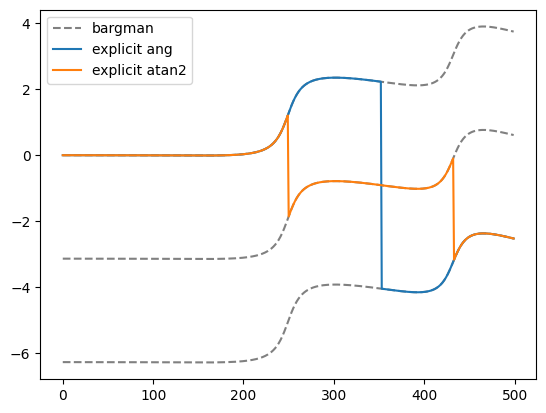
\includegraphics[width = 0.6\textwidth]{fig/premier_resultat}
	\caption[Evolution de la phase géométrique d'un signal AM-FM-PM]{Evolution de la phase géométrique d'un signal AM-FM-PM généré. En gris la phase géométrique du signal calculé via l'invariant de Bargmann. Les deux autres sont calculées avec la formule \cref{eq:phaseg_2var}, en bleu en utilisant de l'argument pour la phase totale et en orange en utilisant atan2.}
\end{figure}

Deux remarques sur ces formules. 
La première est que la phase géométrique ne dépend que des paramètres de polarisations $\theta$ et $\chi$, ce qui reflète son invariance par transformation de jauge.
La seconde, nettement plus troublante, est que $\varphi$ ne s'interprète ni comme phase totale ni comme phase dynamique. 
%Plus loin, \thoughts{\cref{subsec:aller_plus_loin}}, nous reviendrons sur laquelle des deux ``doit'' représenter $\varphi$.
\\
Pour que ce soit le cas, il faut qu'à l'instant $t$ $\x $, retrouve la même polarization instantanée qu'à l'instant $t_0$, auquel cas :
\begin{equation}\label{eq:phases_p-cyc_2var}
	\begin{aligned}
		\big( \chi(t), \theta(t) \big) = \big( \chi(t_0), \theta(t_0) \big)\quad 
		&\Lr\quad \phaset(\x ) = \varphi(t) - \varphi(t) \\
		&\Lr\quad \phaseg(\x ) = -\int_{t_0}^t \theta'(s) \sin 2\chi(s) ds
	\end{aligned}
\end{equation}
\skipl

Ce cas particulier est en fait très instructif puisque qu'il est toujours possible de s't ramener, comme ce sera montrer dans la partie \cref{part:phase_geo} suivante.
\\
Cela étant dit, pour interpréter la formule \eqref{eq:phases_p-cyc_2var} de la phase géométrique, il est utile de d'avoir une représentation de $\x $ qui soit indépendante de sa phase $\varphi$. Représentation ce que nous allons voir à présent.
\\



\subsection{Interprétation dans la sphère de Poincaré}

Ces représentation n'est autre que la matrice de covariance de $\x $ :
\begin{equation} \label{eq:proj2x_2var}
	\forall t\in\R,\quad \rho_{\x}(t) = \frac{1}{\|\x(t) \|^2} \congu{\x(t) }\, ^t\x(t)
\end{equation}
Cette projection, invariante par transformation de jauge, donc indépendante de $\varphi$ et la normalisation est telle que $\rho_{\x}$ ne dépend pas non plus de $a$. La matrice $\rho_{\x}$ ne dépend alors que des paramètres de polarisations, $(\chi, \theta)$, et se décompose dans la base de Pauli suivant :
\begin{equation} \label{eq:decompo_pauli}
	\rho_{\x} = id + \sin(2\theta) \cos(2\chi) \sigma_1 + \sin (2\chi) \sigma_2 + \cos(2\theta) \cos(2\chi) \sigma_3
\end{equation}


\begin{wrapfigure}{r}{0.4\textwidth}
	\begin{tikzpicture}[scale=0.8]
	%\draw[black, opacity=0.1] (-4.5,-4.5) grid (4.5,4.5);
	\draw[-Stealth] (-2.5,0) -- (4.5,0) node[below]{$\sigma_1$};
	\draw[-Stealth] (0,-4.5) -- (0,4.5) node[right]{$\sigma_2$};
	\draw[-Stealth] (2.5,1.2) -- (-2.5,-1.2)  node[below right]{$\sigma_3$};
	
	\coordinate (o) at (0,0);
	\coordinate (i) at (4,0);
	\coordinate (j) at (0,4);
	
	\coordinate (u) at (2.1,2.14);
	\coordinate (p) at (2.1, -0.5);
	\coordinate (v) at (3.4,0.5);
	
	% cercles
	\draw[thick] (4,0) arc [start angle=0, end angle =-140, radius = 4];
	\draw[thick] (4,0) arc [start angle=0, end angle =100, radius = 4];
	
	\draw[thick, dashed] (4,0) arc [start angle=0, end angle =100, radius = 4, y radius = 1];
	\draw[thick] (4,0) arc [start angle=0, end angle =-125, x radius = 4, y radius = 1];
	
	% droites
	\draw[-stealth,thick, blue] (0,0) -- (u) node[above right] {$\rho$};
	\draw[dashed, blue] (u) -- (p);
	\draw[dashed, blue] (0,0) -- (p);
	
	%arc au point
	\draw[gray, dashed] (3.1,2.5) arc [start angle=0, end angle =105, radius = 3.1, y radius = 0.5];
	\draw[gray] (3.1,2.5) arc [start angle=0, end angle =-120, x radius = 3.1, y radius = 0.5];
	
	\draw[violet, -stealth] (-0.4, -0.2) arc [start angle=-120, end angle =-40, x radius = 0.9, y radius = 0.225] node[midway, below] {\scriptsize$2\theta$};    
	\draw[violet, -stealth] (0,0.7) arc [start angle=90, end angle =20, x radius = 0.4, y radius = 0.5];
	\draw[violet] (0.25, 0.8) node{\scriptsize$2\chi$};
\end{tikzpicture}
	\caption{Sphère de Poincaré, blablabla}
	\label{fig:sphere2poincare}
\end{wrapfigure}

\par \noindent
où les $\sigma_i$ sont les matrices de Pauli :
\begin{align*}
	\sigma_1 &= \begin{pmatrix} 0 & 1 \\ 1 &  0 \end{pmatrix}  &
	\sigma_2 &= \begin{pmatrix} 0 & -i \\  i &  0 \end{pmatrix}  &
	\sigma_3 &= \begin{pmatrix} 1 & 0 \\ 0 & -1 \end{pmatrix}
\end{align*}
\skipl

Dans cette décomposition, la composante en $id$ est indépendante de $\x$ et peut donc être ignorée. Cela ne laisse qu'un vecteur (normé) de dimension 3 dont $2\theta$ et $2\chi$ correspondent aux coordonnées polaire conformément à la \Cref{fig:sphere2poincare} ci-contre.
\\ 
\\
La sphère alors obtenue, plus connu sous le nom de sphère de Poincaré, représente l'ensemble des états de polarisation possible pour un signal :
\\
À l'équateur, la polarisation est linéaire et $\theta$ pilote son orientation et plus $\rho_{\x}$ se rapproche des pôles, plus cette polarisation devient elliptique, jusqu'à devenir complètement circulaire, auquel cas $\theta$ devient insignifiant. 
Aussi, suivant le schéma \cref{fig:ellipse2polat}, l'hémisphère nord (resp. sud) correspond à des polarisations elliptiques anti-horaire (resp. horaire).

Le fait que ce soit deux fois les angles qui sont représentés tien naturellement compte des potentielles redondances dans les $(\theta,\chi)$. 
Par exemple si $\x$ à pour paramètre de polarisation instantanée $(\theta_0, \chi_0)$, alors par symétrie de l'ellipse, $(\theta_0+\pi, \chi_0)$ est aussi une représentation valide. Autre exemple, si $\chi_0 = \nicefrac{\pi}{4}$, alors la polarisation est circulaire et indépendant de $\theta_0$.
\\
Dans le deux cas, la représentation dans la sphère de Poincaré évite ces problèmes puisque, dans le premier cas $(2\theta_0, 2\chi_0)$ et $(2\theta_0+2\pi, 2\chi_0)$ représente le même point, et dans le second, le point associé à $2\chi_0=\nicefrac{\pi}{2}$ (pôle nord) est indépendant du choix de $\theta_0$.
\\

\begin{figure}[h]
	
\includegraphics[width=0.8\textwidth]{fig/placeholder}
	\caption{Représentation des paramètres de polarisation instantanée associés à chaque point de la sphère de Poincaré.}
\end{figure}


Pour interpréter la formule \eqref{eq:phases_p-cyc_2var} de la phase géométrique prenons un exemple. Si $\chi$ et $\theta$ sont telle que :
\begin{align*}
	2\theta(t_0) &= 0  &  2\theta(t) &= 2\pi  &  \chi(s) &= \chi_0
\end{align*}
Alors décrit un chemin horizontale sur la sphère, $\rho_{\x}(t_0) = \rho_{\x}(t)$ et sa phase géométrique s'écrit :
\begin{align*}
	\phaseg(\x, t_0, t) = -\int_{t_0}^t \theta'(s) \sin 2\chi(s) ds &= - \sin 2\chi_0 \int_{t_0}^t \theta'(s) ds \\
	&= - \sin 2\chi_0 \big( \theta(t) - \theta(t_0)\big) \\
	&= - \pi\sin 2\chi_0
\end{align*}

Cette formule est très proche de la formule de d'air de la calotte entouré par $\rho_{\x}$, à savoir%\footnote{\itshape
	%La formule se trouve sans mal sur \href{https://fr.wikipedia.org/wiki/Calotte_sph%C3%A9rique#Aire}{Wikipédia}. Dans le lien donné, la formule est fait apparaître un cos, ce qui est dû au choix de convention sur l'angle décrit par $\chi_0$ ($=\nicefrac{\pi}{2} - \theta$ sur Wikipédia)} 
 :
\[\mathcal{A}ire = 2\pi - 2\pi \sin(2\chi_0)\]
Pour la faire clairement apparaître, il suffit de noter que $\phaseg$ étant une phase, elle est définie modulo $2\pi$ et à un facteur 2 près, elle s'écrit :
\begin{align*}
	{\color{white}bbbbbbbbbbbbbbbbbbbbbbbbbbbbbbb}\phaseg(\x, t_0, t) &\equiv 2\pi - \pi\sin 2\chi_0   &  &[2\pi] {\color{white}bbbbbbbbbbbbbbbbbbbbbbbbbbbbbbb} \\
	 &\equiv \frac{1}{2}\big( 4\pi - 2\pi\sin 2\chi_0 \big)    &  &[2\pi] 
\end{align*}

Soit la moitié de l'aire de la calotte au dessus du chemin tracé par $\rho_{\x}$ plus $2\pi$. Une fois n'est pas coutume, ca va toujours pas et j'ai envie de me foutre en l'air atm





\subsection{Généralisation en plus haute dimension} \label{subsec:aller_plus_loin}

\begin{itemize}
	
	\item Différentes écritures du bivarié pour différentes généralisation :
	
	\item Les quaterions on passe vites parce que ca se généralise très mal, Lefevre a a parlée, ca mène aux algèbres Clifford : trop de contrainte sur les dimensions des signaux
	
	\item En terme d'expo de matrice ? Lefevre \cite[sec. I.3]{lefevre_polarization_2021} l'a fait en trivarié mais au delà, y'a plus vraiment de choix remarquable de base pour $\mathfrak{u}(n)$
	
	\item En augmentant la taille de la matrice de rotation ? Lilly \cite{lilly_modulated_2011} l'a fait en trivarié et mais là encore, en terme de généralisation c'est pas si dingue parce que la matrice de rotation est pas calculable.
	
	\item Dans tout ça, on ratte le plus important : La phase géo est invariante par transfo de jauge, donc il faut faut faire apparaître $\PC{n-1}$ dans la décomposition.
	
	\item et en fait, c'est le cas en bivarié car $\PC{1}\cong \S{2}$ !
	
	\item $\PC{n-1}$ oui mais il faut pas non plus regarder que la projection parce qu'on perd toute les phases dans ce cas.
	
	\item Le bon compromis c'est les variétés fibrées : on est dans $\PC{n-1}$ mais on garde les phases dans les fibres.
	
	\item D'autant plus que ça à déjà était fait en physique et c'est vraiment concluant... (transition vers la grande partie suivante.)
	
\end{itemize}

Au niveau des ensembles, décomposer un signal multivarié complexe en paramètre d'amplitude, phase et polarization instantanée, revient à décomposer $\C^n$ en un produit de trois ensembles. Pour cela, un vecteur de $\C^n$ est vu comme la donné d'une direction, \ie~un élément de la sphère unité $S^{2n-1}\subset\C^n$, et d'une norme, de sorte que :
\[\C^n \cong \R^{+_*} \times S^{2n-1}\]
\\
Les éléments de $\R^{+_*}$ s'interprète naturellement comme l'amplitude instantanée du signal et pour faire apparaître sa phase, $S^{2n-1}$ est lui-même décomposé de sorte à faire apparaître $\U{1}$, donnant :
\[\C^n \cong \R^{+_*} \times \U{1} \times S^{2n-1}/\U{1}\]
Le quotient restant n'est autre que l'espace projectif complexe de dimension (complexe) $n-1$, noté $\PC{n-1}$. Sa construction sera détaillée dans la \cref{part:phase_geo} suivante.
\\

Pour motiver d'autant plus cette décomposition, la projection $\rho : \x \lr \congu{\x}\,^t\x / \|\x\|^2$, qui s'est avérée fort instructive, peut être vue comme une projection sur l'espace complexe en cela qu'elles sont toutes deux invariantes par transformation de jauge\footnote{\itshape
	Pour être précis, c'est le premier théorème d'isomorphisme assure $\rho(\C^n) \cong\PC{n-1}$ sont en bijection et de même structure.}.
En particulier, si $n=2$, $\PC{1}\cong S^{2}$, soit exactement l'espace de représentation des $\rho_{\x}$ dans la section précédente.




%%%% ANNEXES %%%%



\begin{annexe}

\section{Annexes}

\subsection{Compléments sur l'analyse temps-fréquence}\label{ann:complement_t-f}

\subsubsection{Un mot sur la notion de fréquence instantanée \thoughts{(nécessaire?)}}\label{ann:freq_instant}

\subsubsection{Formalisme dernière la transformée en SA}\label{ann:transfo_SA}

\subsubsection{Lien avec le théorème de Bedrosian}\label{ann:bedrosian}

\subsection{Compléments sur les signaux AM-FM-PM}\label{ann:AM-FM-PM}

\subsubsection{Construction détaillée des signaux AM-FM-PM \thoughts{(nécessaire?)}}\label{ann:construc_AM-FM-PM}

\begin{itemize}
	
	\item Signal polarisé classique ($\theta,\chi$ constants)
	
	\item Transformé en SA avec les hypothèse de Bedrosian 
	
	\item Définition général en faisant dépendre $\theta / \chi$ du temps
	
	\item Paramètre de Polar sur la sphère de Poincaré
	
\end{itemize}


\subsubsection{Démonstrations}\label{ann:demo_phases_2var}

\begin{demo}[de la formule \eqref{eq:phased_2var}, \cref{prop:phases_2var}]
	Par souci de lisibilité, on note $\ \mathcal{U} = R_{\theta} \begin{pmatrix} \cos\chi \\ -i\sin\chi \end{pmatrix} = \begin{pmatrix} \cos\theta(t) \cos\chi(t) + i\sin\theta(t) \sin\chi(t) \\ \sin\theta(t) \cos\chi(t) - i\cos\theta(t) \sin\chi(t) \end{pmatrix}$, de sorte que la dérivée de $\ \x=ae^{i\varphi}\mathcal{U}\ $ s'écrive :
	\[\dot{\x} = a'e^{i\varphi}\mathcal{U} + ia\varphi'e^{i\varphi} \mathcal{U} + ae^{i\varphi}\theta'\begin{pmatrix} -\sin\theta \cos\chi + i\cos\theta \sin\chi \\ \cos\theta \cos\chi + i\sin\theta \sin\chi \end{pmatrix} + ae^{i\varphi}\chi'\begin{pmatrix} -\cos\theta \sin\chi + i\sin\theta \cos\chi \\ -\sin\theta \sin\chi - i\cos\theta \cos\chi \end{pmatrix}\]
	\\
	Les vecteurs des deux derniers membres s'expriment en fonction des composantes $\ \mathcal{U}_{1,2}\ $ de $\ \mathcal{U}$ :
	\begin{align*}
		\begin{pmatrix} -\sin\theta \cos\chi + i\cos\theta \sin\chi \\ \cos\theta \cos\chi + i\sin\theta \sin\chi \end{pmatrix} &= \begin{pmatrix} -\mathcal{U}_2 \\ \mathcal{U}_1 \end{pmatrix}  &
		\begin{pmatrix} -\cos\theta \sin\chi + i\sin\theta \cos\chi \\ -\sin\theta \sin\chi - i\cos\theta \cos\chi \end{pmatrix} &= i\begin{pmatrix} \congu{\mathcal{U}}_2 \\ -\congu{\mathcal{U}}_1 \end{pmatrix}
	\end{align*}
	\\
	Le produit hermitien $\langle \dot{\x}, \x \rangle$ s'écrit alors :
	\begin{align*}
		\langle \dot{\x}, \x \rangle 
		&= \left\langle a'e^{i\varphi}\mathcal{U} + ia\varphi'e^{i\varphi} \mathcal{U} + ae^{i\varphi}\theta'\begin{pmatrix} -\mathcal{U}_2 \\ \mathcal{U}_1 \end{pmatrix} + iae^{i\varphi}\chi'\begin{pmatrix} \congu{\mathcal{U}}_2 \\ -\congu{\mathcal{U}}_1 \end{pmatrix}, ae^{i\varphi}\mathcal{U} \right\rangle \\
		&= \left\langle a'\mathcal{U} + ia\varphi' \mathcal{U} + a\theta'\begin{pmatrix} -\mathcal{U}_2 \\ \mathcal{U}_1 \end{pmatrix} + ia\chi'\begin{pmatrix} \congu{\mathcal{U}}_2 \\ -\congu{\mathcal{U}}_1 \end{pmatrix}, a\mathcal{U} \right\rangle \\
		&= aa' \big\langle \mathcal{U}, \mathcal{U}\big\rangle  + ia^2\varphi' \big\langle \mathcal{U}, \mathcal{U}\big\rangle  + a^2\theta'\left\langle \begin{pmatrix} -\mathcal{U}_2 \\ \mathcal{U}_1 \end{pmatrix}, \mathcal{U} \right\rangle + ia^2\chi'\left\langle \begin{pmatrix} \congu{\mathcal{U}}_2 \\ -\congu{\mathcal{U}}_1 \end{pmatrix}, \mathcal{U} \right\rangle
	\end{align*}
	où les deux derniers produits hermitiens donnent :
	\begin{align*}
		\left\langle \begin{pmatrix} -\mathcal{U}_2 \\ \mathcal{U}_1 \end{pmatrix}, \mathcal{U} \right\rangle &= -\mathcal{U}_2\congu{\mathcal{U}}_1 + \mathcal{U}_1\congu{\mathcal{U}}_2 \\
		&= 2i\Im m\big(\mathcal{U}_1 \congu{\mathcal{U}}_2\big) \\
		&= 2i\Im m\Big(\big( \cos\theta \cos\chi + i \sin\theta \sin\chi \big) \big( \sin\theta \cos\chi + i \cos\theta \sin\chi \big)\Big) \\
		&= 2i\big(\cos^2\theta \cos\chi \sin\chi + \sin^2\theta \sin\chi \cos\chi \big) \\
		&= 2i \cos\chi \sin\chi \\
		&= i\sin2\chi 
		\\ \\
		\left\langle \begin{pmatrix} \congu{\mathcal{U}}_2 \\ -\congu{\mathcal{U}}_1 \end{pmatrix}, \mathcal{U} \right\rangle &= \congu{\mathcal{U}_2\mathcal{U}_1} - \congu{\mathcal{U}_1\mathcal{U}_2} = 0
	\end{align*}
	\\
	D'où, sachant que $\ \|\x\|^2=a^2\ $ et $\ \|\mathcal{U}\|=1$, la formule :
	\begin{align*}
		\frac{\Im m\big\langle \dot{\x}, \x\big\rangle}{\|\x\|^2} &= \frac{1}{a^2}\Im m\Big(aa' \big\langle \mathcal{U}, \mathcal{U}\big\rangle  + ia^2\varphi' \big\langle \mathcal{U}, \mathcal{U}\big\rangle + ia^2\theta' \sin2\chi \Big) \\
		&= \frac{1}{a^2} \Big( a^2\varphi' \|\mathcal{U}\|^2 + a^2\theta' \sin2\chi \Big) \\
		&= \varphi' + \theta' \sin2\chi
	\end{align*}
\end{demo}

\begin{demo}[de la formule \eqref{eq:phaset_2var}, \cref{prop:phases_2var}]
	Pour la phase totale, on note cette fois $\mathcal{V} = \begin{pmatrix} \cos\chi \\ -i\sin\chi \end{pmatrix}$ et on a :
	\begin{align*}
		\big\langle \x(t), \x(t_0)\big\rangle &= \Big\langle a(t)e^{i\varphi(t)}R_{\theta(t)}\mathcal{V}(t), a(t_0)e^{i\varphi(t_0)}R_{\theta(t_0)}\mathcal{V}(t_0) \Big\rangle \\
		&= a(t)e^{i\varphi(t)} a(t_0)e^{-i\varphi(t_0)} \Big\langle R_{\theta(t)}\mathcal{V}(t), R_{\theta(t_0)}\mathcal{V}(t_0) \Big\rangle \\
		%&= a(t_0)a(t)e^{i(\varphi(t_0)-\varphi(t))}\Big\langle \mathcal{V}(t_0), R_{\theta(t_0)}^{-1}R_{\theta(t)}\mathcal{V}(t) \Big\rangle \\
		&= a(t_0)a(t)e^{i(\varphi(t)-\varphi(t_0))}\Big\langle R_{\theta(t)- \theta(t_0)}\mathcal{V}(t), \mathcal{V}(t_0) \Big\rangle
	\end{align*}
	Pour alléger les notations, on note $\ \Delta y =y(t)-y(t_0)$, $\ y_1=y(t_0)\ $ et $\ y_2=(t)\ $ pour $\ y=\varphi,\theta,\chi$. Le produit hermitien à droite s'écrit alors :
	\begin{align*}
		\Big\langle R_{\Delta\theta}\mathcal{V}(t), \mathcal{V}(t_0) \Big\rangle &=   \Big(\cos\Delta\theta \cos\chi_2 + i\sin\Delta\theta \sin\chi_2 \qquad \sin\Delta\theta \cos\chi_2 - i\cos\Delta\theta \sin\chi_2\Big) \begin{pmatrix} \cos\chi_1 \\ i\sin\chi_1 \end{pmatrix} \\
		&= \cos\chi_1\Big(\cos\Delta\theta \cos\chi_2 + i\sin\Delta\theta \sin\chi_2\Big) + i\sin\chi_1\Big(\sin\Delta\theta \cos\chi_2 - i\cos\Delta\theta \sin\chi_2\Big) \\
		&= \cos\Delta\theta \Big(\cos\chi_1 \cos\chi_2 + \sin\chi_1 \sin\chi_2\Big) + i\sin\Delta\theta \Big( \cos\chi_1 \sin\chi_2 + \sin\chi_1\cos\chi_2\Big) \\
		&= \cos\Delta\theta \cos\Delta\chi + i\sin\Delta\theta \sin(\chi_1+\chi_2)
	\end{align*}
	\\
	D'où la phase totale :
	\begin{align*}
		\phaset(\x) = \arg\big\langle \x(t), \x(t_0)\big\rangle &= \arg\left( a(t_0)a(t)e^{i(\varphi(t) - \varphi(t_0))}\Big( \cos\Delta\theta \cos\Delta\chi + i\sin\Delta\theta \sin(\chi_1+\chi_2) \Big) \right) \\
		&= \varphi(t) - \varphi(t_0) + \arg\Big( \cos\Delta\theta \cos\Delta\chi + i\sin\Delta\theta \sin(\chi_1+\chi_2) \Big)
	\end{align*}
	et l'argument restant s'écrit comme une arctangente, donnant :
	\begin{align*}
		\phaset(\x) &= \varphi(t)-\varphi(t_0) + \arctan\frac{\sin\Delta\theta \sin(\chi_1+\chi_2)}{\cos\Delta\theta \cos\Delta\chi} \\
		&= \varphi(t)-\varphi(t_0) + \arctan \left( \tan\Delta\theta\frac{\sin(\chi_1+\chi_2)}{\cos\Delta\chi} \right) \\
		&= \cdots
	\end{align*}
\end{demo}
\skipl


\subsection{Lien entre Poincaré et Bloch}

\subsubsection{Lien entre les deux types de signaux}

Soit le signal :
\[\x_B(\varphi, \theta, \chi) = e^{i\varphi} \begin{pmatrix}
	\cos \chi/2 \\ e^{i\theta}\sin\chi/2\end{pmatrix}\]
Pour le réécrire en terme de vecteur AM-FM-PM, il faut faire apparaître une matrice de rotation, matrice qui est diagonalisable dans $\C^{n\times n}$ via la relation :
\begin{align*}
	&\begin{pmatrix} 
		\cos \alpha & -\sin \alpha \\ 
		\sin\alpha & \cos\alpha 
	\end{pmatrix} = \frac{1}{2} \begin{pmatrix} 
		1 & -1 \\ i & i
	\end{pmatrix}\begin{pmatrix} 
		e^{-i\alpha} & 0 \\ 
		0 & e^{i\alpha} 
	\end{pmatrix}\begin{pmatrix} 
		1 & -i \\ -1 & -i
	\end{pmatrix}\\
	&\Llr\quad \begin{pmatrix} 
		1 & -i \\ -1 & -i
	\end{pmatrix}\begin{pmatrix} 
		\cos \alpha & -\sin \alpha \\ 
		\sin\alpha & \cos\alpha 
	\end{pmatrix} \begin{pmatrix} 
		1 & -1 \\ i & i
	\end{pmatrix} = 2 \begin{pmatrix} 
		e^{-i\alpha} & 0 \\ 
		0 & e^{i\alpha} 
	\end{pmatrix}
\end{align*}
\\
Cela permet d'écrire :
\begin{align*}
	\x_B(\varphi, \theta, \chi) &= e^{i\varphi} e^{i\theta/2}\begin{pmatrix}
			e^{-i\theta/2} & 0 \\
			0 & e^{i\theta/2}
		\end{pmatrix}\begin{pmatrix} 
			\cos \chi/2 \\ 
			\sin \chi/2 
		\end{pmatrix} \\
		&= \frac{1}{2}e^{i\varphi} e^{i\theta/2}\begin{pmatrix} 
			1 & -i \\
			-1 & -i
		\end{pmatrix}\begin{pmatrix} 
			\cos \theta/2 & -\sin \theta/2 \\ 
			\sin \theta/2 & \cos \theta/2 
		\end{pmatrix} \begin{pmatrix} 
			1 & -1 \\ i & i
		\end{pmatrix}\begin{pmatrix} 
			\cos \chi/2 \\ 
			\sin\chi/2
		\end{pmatrix} \\
		&= \frac{\sqrt{2}}{2}e^{i(\varphi + \theta/2)}U R_{\theta/2} \begin{pmatrix} 
			\cos \chi/2 - \sin\chi/2 \\ 
			i\big(\cos\chi/2 + \sin\chi/2\big)
		\end{pmatrix}   & &\text{où }\quad U = \frac{\sqrt{2}}{2}\begin{pmatrix} 
		1 & -i \\ -1 & -i
		\end{pmatrix}\in \U{2} \\
\end{align*}
\\
Ensuite, pour réduire les sommes dans le vecteur de droite, on a rappel les formules :
\begin{align*}
	\cos\left( \frac{\pi}{2} \pm \alpha\right) &= \frac{\sqrt{2}}{2}\big( \cos\alpha \mp \sin \alpha \big) & \sin\left( \frac{\pi}{2} \pm \alpha\right) &= \frac{\sqrt{2}}{2}\big( \cos\alpha \pm \sin \alpha \big)
\end{align*}
\\ 
On a donc deux choix pour chaque composante du vecteur mais celle avec un signe moins son préférable sachant que : 
\begin{align*}
	\cos\left( \frac{\pi}{2} - \alpha\right) &= \sin(\alpha) &  \sin\left( \frac{\pi}{2} - \alpha\right) &= \cos(\alpha)
\end{align*}
\\
On choisi donc la seconde formule pour la première composante et la premier pour la seconde composante, donnant :
\begin{align*}
	\x_B(\varphi, \theta, \chi) &= \frac{\sqrt{2}}{2}e^{i(\varphi + \theta/2)}U R_{\theta/2} \begin{pmatrix} 
		\cos \chi/2 - \sin\chi/2 \\ 
		i\big(\cos\chi/2 + \sin\chi/2\big)
	\end{pmatrix} \\
	&= e^{i(\varphi + \theta/2)}U R_{\theta/2} \begin{pmatrix} 
		\sin\left( \frac{\pi}{2} - \chi/2\right) \\ 
		i\cos\left( \frac{\pi}{2} - \chi/2\right)
	\end{pmatrix} \\
	&= e^{i(\varphi + \theta/2)}U R_{\theta/2} \begin{pmatrix} 
		\cos \chi/2 \\ 
		i\sin \chi/2
	\end{pmatrix}
\end{align*}
\\
Ne reste alors plus qu'à ajuster les signes pour obtenir une écriture de signal $\x_P$ AM-FM-PM :
\begin{align*}
	\x_B(\varphi, \theta, \chi) &= e^{i(\varphi + \theta/2)}U R_{\theta/2} \begin{pmatrix} 
		\cos \chi/2 \\ 
		i\sin \chi/2
	\end{pmatrix} \\
	&= U e^{i(\varphi + \theta/2)} R_{\theta/2} \begin{pmatrix} 
		\cos (-\chi/2) \\ 
		-i\sin (-\chi/2)
	\end{pmatrix}
\end{align*}
En somme :
\begin{align} \label{eq:bloch2poinca}
	\x_B(\psi, \alpha, \beta) &= U \x_P(\psi + \alpha/2, \alpha/2, -\beta/2)  & 
	\x_P(\varphi, \theta, \chi) = U^\dagger 	\x_B(\varphi-\theta, 2\theta, -2\chi)	
\end{align}
\skipl 



\subsubsection{Lien entre les projections}

Avec la formule \eqref{eq:bloch2poinca} ci-dessus, on a :

\begin{align}
	\rho_B(\alpha, \beta) &= U \rho_P(\alpha/2, -\beta/2)U^\dagger  & 
	\rho_P(\theta, \chi) &= U^\dagger \rho_B(2\theta, -2\chi) U
	%\\ \Llr\ \rho_B(\alpha, \beta) U &= U \rho_P(\alpha/2, -\beta/2) & \Llr\ \rho_P(\theta, \chi) U^\dagger &= U^\dagger \rho_B(2\theta, -2\chi) 
\end{align}
\\
Mais on a aussi, dans la base Pauli :
\begin{align*}
	\sigma_1 &= \begin{pmatrix} 0 & 1 \\ 1 &  0 \end{pmatrix}  &
	\sigma_2 &= \begin{pmatrix} 0 & -i \\  i &  0 \end{pmatrix}  &
	\sigma_3 &= \begin{pmatrix} 1 & 0 \\ 0 & -1 \end{pmatrix}
\end{align*}
les expressions :
\begin{align*}
	\rho_{P}(\theta, \chi) &= \frac{1}{2} \Big( id + \sin(2\theta) \cos(2\chi) \sigma_1 - \sin (2\chi) \sigma_2 + \cos(2\theta) \cos(2\chi) \sigma_3 \Big) \\ 
	\rho_{B}(\alpha, \beta) &= \frac{1}{2} \Big( id + \cos(\alpha) \sin(\beta) \sigma_1 + \sin(\alpha) \sin(\beta) \sigma_2 + \cos (\beta) \sigma_3 \Big)
\end{align*}
\skipl

Pour les lier, on pose $\ 2\theta = \nicefrac{\pi}{2} - \alpha\ $ et $\ 2\chi = \nicefrac{\pi}{2} - \beta$, donnant :
\begin{align*}
\rho_P(\theta, \chi) - id 
	&= \sin(\nicefrac{\pi}{2} - \alpha) \cos(\nicefrac{\pi}{2} - \beta) \sigma_1 - \sin (\nicefrac{\pi}{2} - \beta) \sigma_2 + \cos(\nicefrac{\pi}{2} - \alpha) \cos(\nicefrac{\pi}{2} - \beta) \sigma_3 \\
	&= \cos(\alpha) \sin(\beta) \sigma_1 - \cos (\beta) \sigma_2 + \sin(\alpha) \sin(\beta) \sigma_3
\end{align*}
\\
Ce qui sous forme matricielle se réécrit :
\[\begin{pmatrix}
	\sin(2\theta) \cos(2\chi) \\ -\sin (2\chi) \\ \cos(2\theta) \cos(2\chi)
\end{pmatrix} = \begin{pmatrix}
	\cos(\alpha) \sin(\beta) \\ -\cos (\beta) \\ \sin(\alpha) \sin(\beta)
\end{pmatrix} = \begin{pmatrix}
	1 & 0 & 0 \\ 0 & 0 & -1 \\ 0 & 1 & 0
\end{pmatrix}\begin{pmatrix}
	\cos(\alpha) \sin(\beta) \\ \sin(\alpha) \sin(\beta) \\ \cos (\beta)
\end{pmatrix}\]
\\
Donc la passage de $\rho_B$ à $\rho_S$ se fait via un changement et d'angle et une rotation de $\nicefrac{\pi}{2}$ autour de $\sigma_1$.
\\

Même calcul, cette fois, en partant de \eqref{eq:bloch2poinca} :
\begin{align*}
	2\rho_P(\theta, \chi) &= 2U^\dagger \rho_B(2\theta, -2\chi) U \\
	&= U^\dagger \Big( id + \cos(2\theta) \sin(-2\chi) \sigma_1 + \sin(2\theta) \sin(-2\chi) \sigma_2 + \cos (-2\chi) \sigma_3 \Big) U \\
	&= id - \cos(2\theta) \sin(2\chi) U^\dagger \sigma_1 U - \sin(2\theta) \sin(2\chi) U^\dagger \sigma_2 U + \cos (2\chi) U^\dagger \sigma_3 U
\end{align*}
avec :
\begin{align*}
	U^\dagger \sigma_1 U &= \frac{1}{2} \begin{pmatrix} 
		1 & -1 \\ i & i
	\end{pmatrix} \begin{pmatrix} 
		0 & 1 \\ 1 &  0 
	\end{pmatrix} \begin{pmatrix} 
		1 & -i \\ -1 & -i
	\end{pmatrix} = \frac{1}{2} \begin{pmatrix} 
		-2 & 0 \\ 0 & 2
	\end{pmatrix} = -\sigma_3 \\
	U^\dagger \sigma_2 U &= \frac{1}{2} \begin{pmatrix} 
		1 & -1 \\ i & i
	\end{pmatrix} \begin{pmatrix} 
		0 & -i \\  i &  0 
	\end{pmatrix} \begin{pmatrix} 
		1 & -i \\ -1 & -i
	\end{pmatrix} = \frac{1}{2} \begin{pmatrix} 
		0 & -2 \\ -2 & 0
	\end{pmatrix} = -\sigma_1 \\
	U^\dagger \sigma_3 U &= \frac{1}{2} \begin{pmatrix} 
		1 & -1 \\ i & i
	\end{pmatrix}  \begin{pmatrix} 
		1 & 0 \\ 0 & -1 
	\end{pmatrix} \begin{pmatrix} 
		1 & -i \\ -1 & -i
	\end{pmatrix} = \frac{1}{2} \begin{pmatrix} 
		0 & -2i \\ 2i & 0
	\end{pmatrix} = \sigma_2
\end{align*}
\\
Qui donne :
\begin{align*}
	2\rho_P(\theta, \chi) &= id - \cos(2\theta) \sin(2\chi) U^\dagger \sigma_1 U - \sin(2\theta) \sin(2\chi) U^\dagger \sigma_2 U + \cos (2\chi) U^\dagger \sigma_3 U \\
	&= id + \cos(2\theta) \sin(-2\chi) \sigma_3 + \sin(2\theta) \sin(-2\chi)  \sigma_1 + \cos (-2\chi) \sigma_2 \\
	&= id + \sin(2\theta) \sin(2\chi)  \sigma_1 + \cos (2\chi) \sigma_2 + \cos(2\theta) \sin(2\chi) \sigma_3
\end{align*}
\\ 
Le tout reste cohérent et avec les notations :
\begin{align*}
	w_P(\theta, \chi) &= \begin{pmatrix}
		\sin(\theta) \cos(\chi) \\ -\sin (\chi) \\ \cos(\theta) \cos(\chi)
	\end{pmatrix}  &   w_B\big( \alpha, \beta \big) = \begin{pmatrix}
		\cos(\alpha) \sin(\beta) \\ \sin(\alpha) \sin(\beta) \\ \cos (\beta)
	\end{pmatrix}
\end{align*}
Cela devient :
\[w_P(2\theta, 2\chi) = \begin{pmatrix}
	1 & 0 & 0 \\ 0 & 0 & -1 \\ 0 & 1 & 0
\end{pmatrix} w_B\big( (\nicefrac{\pi}{2}-\theta ), \big(\nicefrac{\pi}{2}-\chi) \big)\]
\skipl 



\subsubsection{Transformation de phases}

Première chose, le produit hermitien est invariant par $U\in\U{2}$ (si si). Ainsi :
\[\big\langle U\x(t_0), U\x(t) \big\rangle = \big\langle \x(t_0), \x(t) \big\rangle\]
\[\big\langle (U\x)', U\x \big\rangle = \big\langle U\x', U\x \big\rangle = \big\langle \x', \x \big\rangle\]
\\
Ainsi, en utilisant les formules \eqref{eq:phaset_2var} et \eqref{eq:bloch2poinca}, on a :
\begin{align*}\phaset \big(\x_B(\psi, \alpha, \beta) \big) &= \phaset \big(\x_P(\psi + \alpha/2, \alpha/2, -\beta/2) \big) \\
	&= \big( \psi + \alpha/2 \big)(t) - \big( \psi + \alpha/2 \big)(t_0) - \arctan\left( \tan \frac{\Delta\theta}{2} \frac{ \tan 2\beta(t_0)+\tan 2\chi(t)}{1 + \tan 2\beta(t_0)\tan 2\beta(t)}\right)
\end{align*}
Mais avec un calcul immédiat, on a aussi :
\[aoerinagrqobne\]
\\
Avec la formule de la phase dynamique dans Poincaré \eqref{eq:phased_2var}, on a :
\begin{align*}
	%\phaset \big(\x_B(\psi, \alpha, \beta) \big) &= \phaset \big(\x_P(\psi + \alpha/2, \alpha/2, -\beta/2) \big) 
	%\\ \\
	\phased \big(\x_B(\psi, \alpha, \beta) \big) &= \Im m \int_{t_0}^t \left\langle \frac{d}{ds}\x_B(\psi, \alpha, \beta), \x_B(\psi, \alpha, \beta) \right\rangle ds \\
	&= \Im m \int_{t_0}^t \left\langle \frac{d}{ds}\x_P(\psi + \alpha/2, \alpha/2, -\beta/2), \x_P(\psi + \alpha/2, \alpha/2, -\beta/2) \right\rangle ds \\
	&= \phased \big( \x_P(\psi + \alpha/2, \alpha/2, -\beta/2) \big) \\
	&= \psi(t) + \alpha(t)/2 - \big( \psi(t_0) + \alpha(t_0)/2 \big) - \int_{t_0}^t \frac{\alpha'(s)}{2} \sin \big( -2\beta(s)/2 \big) ds \\
	&= \psi(t) - \psi(t_0) + \frac{\alpha(t) - \alpha(t_0)}{2} + \frac{1}{2} \int_{t_0}^t \alpha'(s)\sin \beta(s) ds
\end{align*}
\\
Mais dans le même temps, si on calcul la phase dynamique de $\x_B$, on tombe cette fois sur :
\begin{align*}
	\phased\big(\x_B(\psi, \alpha, \beta) \big) &= \psi(t) - \psi(t_0) +  \int_{t_0}^t \alpha'(s) \frac{1 - \cos\beta(s)}{2}ds \\
	&= \psi(t) - \psi(t_0) + \frac{\alpha(t) - \alpha(t_0)}{2}- \frac{1}{2} \int_{t_0}^t \alpha'(s) \cos\beta(s) ds 
\end{align*}
Auquel cas :
\begin{align*}
	\phased\big(\x_S(\varphi, \theta, \chi) \big) &= \phased\big(\x_B(\varphi-\theta, 2\theta, -2\chi) \big) \\
	&= \varphi(t) - \theta(t) - \big( \varphi(t_0) - \theta(t_0) \big) + \frac{1}{2} \int_{t_0}^t 2\theta' (1 - \cos2\chi)ds \\
	&= \varphi(t) - \varphi(t_0) - \big( \theta(t) - \theta(t_0) \big) + \int_{t_0}^t \theta' (1 - \cos2\chi)ds \\
	&= \varphi(t) - \varphi(t_0) - \big( \theta(t) - \theta(t_0) \big) + \big( \theta(t) - \theta(t_0) \big) - \int_{t_0}^t \theta' \cos2\chi ds \\
	&= \varphi(t) - \varphi(t_0) - \int_{t_0}^t \theta' \cos2\chi ds
\end{align*}
Ce qui voudrait dire que :
\[\phased\big(\x_S(\varphi, \theta, \chi) \big) = \varphi(t) - \varphi(t_0) + \int_{t_0}^t \theta' \sin2\chi ds = \varphi(t) - \varphi(t_0) - \int_{t_0}^t \theta' \cos2\chi ds\]
... bizarre


\end{annexe}